\documentclass[a4paper,12pt]{article} %style de document                        
\usepackage[utf8]{inputenc} %encodage des caractères                            
\usepackage[french]{babel} %paquet de langue français                           
\usepackage[T1]{fontenc} %encodage de la police                                 
\usepackage[top=2cm,bottom=2cm,left=2cm,right=2cm]{geometry} %marges            
\usepackage{graphicx} %'affichage des images                                    
\usepackage{verbatim}
\frenchbsetup{StandardLists=true}
\usepackage{enumitem}
\usepackage{amssymb}
\usepackage{perpage}
\MakePerPage{footnote}
\usepackage{hyperref}
\begin{document}
\renewcommand{\contentsname}{Sommaire}
\title{Projet Bataille naval}
\author{Céleste \textsc{Le Pifre}, Albert \textsc{Peltier}, Guillaume \textsc{Lericheux}}
\date{2023}
\maketitle
\begin{center}

\includegraphics[scale=0.5]{UNICAEN.png}
\end{center}
\section{Introduction}
Dans le cadre de notre projet de fin de semestre, sur la bataille navale avec un modèle MVC, nous écrivons ce rapport où nous expliquerons notre démarche et où nous développerons la façon dont nous avons pensé ce projet. Pour commencé nous allons vous dire quel sont les règles que nous avons utilisé pour le jeu : 
- Premièrement le jeu contient deux joueurs , le premier étant un humain (vous en l'occurrence ) , le second est un robot qui va jouer des coups aléatoirement.
- Deuxièmement le jeu possède les particularités suivantes :
\begin{itemize}
\item Deux bateaux ne peuvent pas être cote à cote.
\item Si un joueur peut taper deux fois à la même coordonnée , néanmoins sont tour sera donc vide/inutile .
\item Lorsqu'un bateau coule il est entouré d'un rectangle arrondi / est indique dans le terminal pour prevenir le joueur.
\item Un coup en dehors de la grille n'est pas comptabilisé et le joueur doit rejouer.
\item Si un coup touche , le joueur ne peut pas rejouer et c'est au tour du joueur adverse , il en est de même si le coup est raté .
\item Lorsqu'un joueur touche tout les bateaux de l'adversaire la partie s'arrête , elle annonce le nom du vainqueur et demande si le joueur(humain) souhaite refaire une partie .
\end{itemize}
\newpage
\tableofcontents
\section{MVC}
\subsection{But du projet en MVC}
Dans notre cours d'Interfaces Graphiques et Design, la création d'un modèle MVC nous semblait compliquée. En effet, cela nécessitait une rigueur de code à laquelle nous n'étions pas habitués, ce qui rendait l'apprentissage difficile. De plus, les TP ne contenaient que de petits exercices que nous pouvions facilement terminer en 4 à 6 heures. Par conséquent, nous pensions que cela était peu utile et contraignant cependant la présence du mvc comptant pour une grande  partie de la note , nous a forcés à l'utiliser .

Nous avons alors réalisé que l'utilisation du modèle MVC était évidente et qu'il apportait de nombreux avantages. Grâce à sa structure, nous avons pu mieux répartir les tâches entre les membres du groupe et travailler plus efficacement ensemble. De plus, cela a permis une meilleure compréhension du code et une plus grande adaptabilité pour les modifications futures. En fin de compte, nous avons compris l'importance de la rigueur de code et de la structure dans un projet de grande envergure.
 
\subsection{Comment fonctionne le MVC}

Le MVC(Modèle-Vue-Contrôleur) est une manière de programmé très utilisé, on doit alors séparé trois partie principales Modèle, Vue et contrôleur.
\begin{itemize}
\item Le Modèle contient la logique de l'application, c'est-à-dire les règles du programme qui sont des méthodes et des fonctions, mais ne sais pas les utilisé ni les instancié. Dans d'autre utilisation notamment dans le monde professionnelle, il peut aussi géré l'accès au données. Le modèle est aussi indépendant c'est à dire qu'il ne dépend ni de la Vue ni du contrôleur.

\item La Vue occupe de l'interface utilisateur elle est chargé de partagé les données à l'utilisateur et de collecté ses entrées : clic de souris, frappes de clavier, etc... ; elle transmettra par la suite ces information au Contrôleur pour qu'il puisse les téter. La Vue est donc dépendent du Modèle, car elle à besoin de cherché les données dans ce dernier, mais pas du Contrôleur car elle n'a pas à savoir la logique de l'application.

\item Le Contrôleur écoute les événements de la vue, comme les clic souris, puis  effectue les actions nécessaires en fonction de ces événements. Il peut également mettre à jour la vue en fonction des changements effectué. Il peut également effectuer des opérations de validation et de vérification des données entrées par l'utilisateur, afin de garantir que ces données sont correctes et conformes aux règles définies par le modèle.
\end{itemize}

Ainsi le MVC permet de faire séparation du code pour une meilleure lisibilité et répartition du code.
Pour faire une analogie avec le corps humain le Modèle serais le corps la Vue serais les sens et le Contrôleur serais le cerveau 


\section{Modele}
\subsection{Plan du modele}
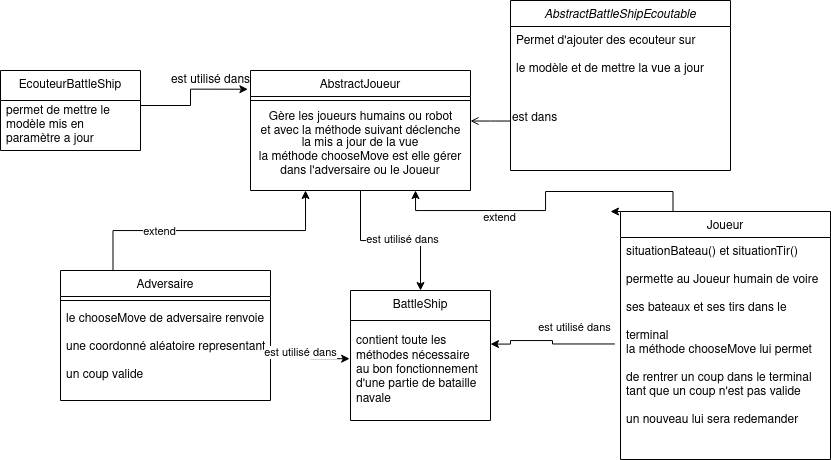
\includegraphics[scale=0.5]{Diagramme.png}
\subsubsection{AbstractJoueur}
Cette class contient les méthodes commune aux deux joueurs (Joueur et Adversaire ). Les méthodes les plus notables de cette class sont:
\begin{itemize}
\item misAjourFlotte() qui permet d'enlever les bateaux coulés de la liste et de les mettre dans la liste bateauQuiNagentAvecLesPoissons qui represente la liste des bateaux coulé cette liste est utile à la vue
\item modifieGrille() et modifieAffichage() qui permettent de mettre a jour les grilles du joueur a une certaines coordonées. Grâce à cela on peut voir si un bateau a été touché ou si un tir a été manqué par exemple. Les grilles étant modifié on effectue les tests sur les grilles des joueurs pour savoir où sont leur bateaux et si ils sont touchés.
\item coupGraphique() cette méthode permet de récupérer une coordonnée et de l'ajouter à coupsJouer si elle n'est pas null. C'est elle qui donne sa valeur à coupGraphique. Ce  sera utile lors de la
gestion de partie Graphique. 
\end{itemize}
\subsubsection{Creation des 2 instances Joueurs}
Nous avons créées deux class Joueur et Adversaire les deux héritent de la class abstraite AbstractJoueur. Le Joueur a deux méthodes en plus qui lui permette de visualiser ses tirs et l'états de ces bateaux. Sinon les deux class réecrivent la fonction chooseMove(). L'Adversaire fait en sorte qu'elle renvoie un coup aléatoire et le Joueur quand a lui demande de choisir un coup dans le terminal
puis verifie sa validité grâce à la méthode verifieCoup() dans BattleShip.
\subsubsection{BattleShip}
BattleShip est la class qui contient toutes les méthodes necessaires à une partie de bataille navale. Les méthodes les plus notables de cette class sont:
\begin{itemize}
\item verifpositionnement() qui prend en paramètre une coordonnés, un sens, et une taille. Soit tous les paramètres d'un bateau. Pour chaque case qui compose le potentiel futur bateau on utilise la méthode placementBateauValid() qui vérifie a l'aide de la latitude et de la longitude d'une Coordonnée que un bateau peut bien être placé. On verifie qu'il soit bien dans la grille et qu'il ne soit
pas sur un autre bateau. Une boucle for parcours toutes les cases qui composeront le potentiel futur bateau en les faisait toutes passée par placementBateauValid(). Lors de cette boucle if on s'assure aussi qu'il n'y a pas de bateau à moins d'une case de celui que on essaie de creer car a la méthodes pointAutour() qui nous dit si des bateaux sont présent autour. Si les paramètre entrée peuvent permettrent la création d'un bateau alors on renvoie true et dans la méthode qui a a fait appel a verifpositionnment() un nouveau bateau sera créée. 
\item creeFlotteRandom() cette méthode permet de créer une flotte aléatoirement. Elle crée la flotte des deux joueurs en début de partie. Pour cela on génère des coordonnées aleéatoire et un booleen nous donne le sens du bateau. Ensuite on verfie si on utlise la méthode verifpositionnement() pour voir si on peut créer un bateau avec les coordonnées générés et le sens proposé. Si true est renvoyé alors on ajoute le bateau à la flotte du joueur actuel. Dans le controleur le joueur sera changé et on créera une flotte aléatoire pour le joueur suivant.
\item verifieCoup() permet de s'assurer que le string recupérer par le scanner et dont la valeur a été attribuer par le Joueur humain lors d'un chooseMove represente bien un coup valide. Grâce a cette méthode on ne peut pas mettre de lettre ou tiré en dehors de la grille.
\item partieFini() est utilisé pour arreté la partie. Elle renvoie false tant que tous les joueurs ont encore au moins un bateau. Quand un des joueur n'a plus de bateau dans sa flotte la partie 
s'arrête.
\item coup() permet de jouer tirer sur la grille de bateau du joueur dont c'est pas le tour et de mettre la grille de tir du joueur actuel à jour. En modifiant la grille à l'endoit du tir. 
\end{itemize}
\subsection{Bateau et Coordonner}
Bateau est une liste de Coordoner avec un sens et la Coordonner qui a permis sa création. Le bateau génère lui même sa liste de coordonnées car a celle de départ et un sens. Bateau possède la methode tirSurBateau() qui suprime les Coordonner de la liste a l'endroit où le bateau est touché. La méthode coule() elle permet de savoir quand un Bateau n'a plus de Coordoner dans sa liste de Coordonner (quand toutes ses cases se sont fait touchées). Cette méthode sert lors de la misAjourFlotte().\\
La class Coordonner possède juste une latitude et une longitude.   
\subsubsection{Implementation du MVC depuis le modele}
Le modèle se gère tout seul avec le controleur, il ne nécessite pas la vue. Une partie entière peut être gérer indépendamment. Pour l'implémenter au modèle mvc nous avons utilisé des écouteurs.


\section{Vue}
La conception de la vue est importante car elle permet de rendre le jeux plus accueillant que sur un terminal de commande , il fallait donc implémenter des fonctionnalité intuitive pour le joueur telle que :
\begin{itemize}
\item Une distinction rond rouge , rond vert si la case est un bateau ou non .
\item Un rectangle arrondit qui se déploie autour d'un bateau totalement coulé afin de faire comprendre au joueur qu'il a coulé.
\item La fonctionnalité qui permet de cliquer sur la grille adverse afin d’exécuter un coup .
\item Et l'apparition de deux "pop up" qui permettent respectivement de recuperer le nom du joueur et de  relancer une partie sans passer par le terminal.
\end{itemize}
Toute ces fonctionnalités ont été rassemblé dans le dossier Vue contenant 4 fichiers qui permettent de mettre en place tout ce qui a été cité précédemment.
Bien évidemment aucune de ces fichier ne part modifier les fonctions du modèle afin d'obtenir un modèle MVC ou le modèle est indépendant de la Vue .
\subsection{L'implementation du Mvc depuis la Vue}
Comme vu précédemment dans l'onglet "Implementation du MVC depuis le modele" une interface nommée "EcouteurBattleShip.java" à été créer contenant la fonction modeleMisAJour .
Notre Vue , et plus précisément le Jpanel , va hériter de l'interface afin de récupérer les états de la partie de jeux(BattleShip).
Dans la classe qui hérite "ecouteurbattleShip" on va donc Override   la méthode "ModeleMisAJour" (par obligation des interfaces). 

Ce qui signifie que des que la fonction "firechangement" sera exécute la fonction "modeleMisAjour" le sera elle aussi sur tout les éléments de l'ecouteurBattleShip .

Le modeleMisAJour Override du Jpanel vaut donc un repaint ce qui permet de redessiner comme son nom l'indique , chaque élément de EcouteurBattleShip.

Pour résumé, cela signifie que chaque fois que la fonction suivant() est utilisé cela actualise le Jpanel en question .   

\subsection{Jframe}
Le Jframe lui contient une instance de BattleShip (la classe qui supervise la partie de bataille navale) avec ses deux joueurs.

Grace à cela la vue peut accéder à littéralement 95 pourcent des fonctions et des variables placée dans le modèle.

Le plus important dans cette classe est la creation de deux instances de la même classe Jpanel -> le BattleShipJpanel .
Seule les arguments du battleShipJpanel changent mais tout ceci sera expliqué plus précisément dans la partie dédié au Jpanel .

En ce qui concerne le BorderLayout c'est assez simple il y a :
\begin{itemize}
\item Un BorderLayout.CENTER qui permet de mettre un Jpanel sur la gauche du Jframe .
\item Un BorderLayout.EAST qui permet de mettre un Jpanel sur la droite du Jframe.
\end{itemize}


\subsection{Jpanel}
Le Jpanel est la partie la plus fournit de la vue , cela a du sens étant donné qu'il contient les deux grilles de jeux avec de nombreuse méthodes  .

Avant de commencer il faut déjà avoir plusieurs points en tête lorsque que l'on manie/parle de ce Jpanel.
\begin{itemize}
\item Premièrement : La classe BattleShipJpanel est la même que l'on utilise pour représenter le joueur ou bien le robot .
Cela permet de factoriser le code en un seul emplacement plutôt que d'avoir deux classe Jpanel pour les différencier .
Le moyen le plus simple pour faire en sorte que le code s’exécute pour un seul joueur est de : 
Comparer la valeur de l'abstract Joueur donné en argument dans le constructeur du Jpanel avec la valeur que l'on souhaite obtenir dans le BattleShip prit lui aussi en argument.
exemple :<insere une image de Jpanel ligne 88>
\item Deuxiemement : La Classe Jpanel pour afficher des éléments à l'image via Swing utilise un PaintComponent.
Cela signifie que à chaque repaint utilisé lorque la fonction suivant() est utilisé (voir L'implementation du Mvc depuis la Vue), il faut redessiner TOUT ce qui doit être afficher.
Et non pas uniquement les nouveaux éléments qui sont apparue avec un nouveau coup par exemple .
Cela explique la nombreuse présence d'ArrayList qui permettent de stocker de nombreuse valeurs .
\item Dernièrement la taille de chaque grille de jeux et de TOUT ses éléments (rond ,rectangle arrondie ect ...) est basé sur un "private final static int " nommé dim .
Normalement il vaut 60 mais le changer ne posera pas de problème car TOUT est en proportion de dim il n'y aura donc aucun problème graphique en ce qui concerne la taille des éléments des Jpanels .
\end{itemize}

Il est temps de rentrer dans le vif du sujet :

\subsubsection{Le PaintComponent}
Le paintcomponent commence par dessiner en premier lieux ce qui ne va pas changer au fil de la partie  , c'est a dire tout ce qui est en dehors des grilles on y retrouve donc :
\begin{itemize}
\item Les lettres de "A" à "J" placé de gauche à droit en haut de la grille. 
\item Les Chiffres de 1 à 10 placé de Haut en Bas de la grille.
Ces deux éléments permettent d'aider le joueur à savoir ou tirer .
\item Le rectangle qui détermine la taille de la grille il est de valeur dim jusqu’à dim*10 . (rappel changer la valeur de dim modifie la valeur de tout les éléments cela ne pose donc pas de problème).
\item Le quadrillage de la grille afin d'aider le joueur à cliquer la ou il le souhaite .
\end{itemize}
\subsubsection{Afficher les bateaux alliés}
Dans L’énoncé du projet on peux voir sur la partie graphique que le joueur peux voir ses bateaux en debut de partie , alors que les bateaux du robot eux ne le sont pas .

Cela crée donc une différence d'affichage entre la grille de droite et la grille de gauche alors que je le rappel qu'on utilise le meme Jpanel.
La solution se situe ligne 88 ou cela me permet de "Paint " uniquement sur la partie du joueur.
Enfin pour la fonction en elle même elle est assez basique :
-Je recupere la liste bateau du joueur ligne 89.
-Je le parcours ligne 90.
-En fonction de son sens je dessine un carré arrondie sur les cotés ligne 92.
\subsubsection{Les Coups executés}
Les coups exécuté par le joueur et le robot sont récupéré dans le modèle , plus précisément dans la classe abstractJoueur.

Ensuite les coups sont stockées dans l'ArrayList coupsJouer. On recupère cette liste et on la parcours. A chaque position on regarde si le coup avait touché un bateau ou non, pour cela on regarde l'état du la grille de bateau (de l'AbstractJoueur qui s'est fait tiré dessus) a la position du coup (ligne 74). En fonction de cela le point correspondant au coup sera en rouge ou en vert.
\subsubsection{L'action Listener de la souris}\label{coupGraphique}
Pour terminer , il faut laisser la possibilité au joueur de cliquer sur la grille adverse afin de faire l'équivalent de la fonction coup dans le terminal.

On veut bien évidemment ne pas laisser la possibilité au joueur de cliquer sur sa propre grille afin de faire un coup , ce qui explique la présence de la ligne 25.

Pour ce qui s'agit du reste ce n'est rien de bien compliqué il s'agit juste de la fonction mouseListener et de ses methodes. 

Il y a juste une petite particularité les coordonnées du click sont decrementé de 1 car pour le Jpanel les valeur (0,0) (0,1) (1,0) etc sont cliquable mais c'est un clic en dehors de la grille donc le coup n'est pas pris en compte (On clique à l'endroit ou il a les 10 chiffres et caractères ).

Les coups reçu par le clique de souris sont envoyer au Joueur pour qu'ils puissent être joué. Si le coup est null il ne se passe rien. Le coup n'est pas ajouter à l'Arraylist des coupsJouer et la valeur de coupGraphique restera null (ce qui a pour conséquence  de nous permettre d'attendre un nouveau coup). 

\section{Controleur}

\subsection{Orchestrator}
La class Orchestrator contient le Main dont on verra après le fonctionnement et deux méthodes, getJouer() et play(). Orchestrator dans sont ensemble permet de créer et de gérer la partie de bataille navale.
\subsubsection{getJouer()}
La méthode getJouer() permet de retourner la valeur de jouer de l'Ochestrator. A la création de l'Orchestrator jouer vaut 1. A la fin du main la valeur de jouer du main vaut la valeur de jouer de l'Orchestrator.
\subsubsection{play(int affichage)}
Cette méthode est celle qui gère la partie. Elle prend en paramètre un entier représentant le type d'affichage choisi dans le main (voir \ref{affichage}).
\newline
\paragraph{Partie Graphique}Si l'on a choisie de jouer avec une interface graphique la gestion de la partie ce fait différemment. Tout d’abord on crée et affiche la fenêtre de jeu. Ensuite on rentre dans la boucle de jeu (on n'en sort que lorsque la partie se termine).On commence par changer le joueur courant avec la méthode changePlayer() de BattleShip. A chaque tour on regarde si c'est le joueur ou le robot qui joue. En fonction de cela différente valeur sont attribuer à coup (Une coordonnées représentant le coup à jouer).
\begin{itemize}
\item Si c'est l'Adversaire (robot) coups est défini par le retour de la fonction chooseMove de l'Adversaire(robot). Le coup est donc aléatoire.
\item Si c'est le joueur(humain) on rentre dans une boucle while qui attend que le coupGraphique du Joueur soit différent de null. Puis on recupère le coupGraphique dans coups. Le coupGraphique prend sa valeur depuis un click du Joueur (voir \ref{coupGraphique}).
\end{itemize}
coups est ensuite joué dans le modèle, on exécute la méthode suivant de L'abstractJoueur dont c'était le tour (on met la vue à jour), et enfin coupGraphique est réinitialiser pour le prochain tour du joueur. Ces actions se déroulent jusqu’à ce que la partie soit fini (ligne 30). A la fin de la partie la fenêtre de jeu se ferme et une nouvelle affichant le gagnant nous propose de rejouer.
En cliquant sur oui on met la variable jouer de l'Orchestrator à 1, en cliquant sur non on la met à 2. Cette variable est réutilisée après dans le main. 
\paragraph{Partie dans le terminal}
Au début de la partie dans le terminal on entre aussi dans la boucle de jeu (ligne 55), don on ressort que lorsque que la partie est fini. A chaque itération de boucle (qui corresponde chacune au tour de un joueur (Joueur ou Adversaire) on change de joueur. Puis on demande le coup a jouer via chooseMove du jactuel (joueur dont c'est le tour). Une fois le coup choisi il est exécuté avec la méthode coup de BattleShip. A la fin de partie le gagnant s'affiche et on demande dans le terminal si on veut rejouer. Si on entre 1 une nouvelle partie démarre et si on entre 2 le programme s'arrête (Si aucune des deux valeur est entré on repose la question). Comme lors la partie Graphique la valeur entré est attribuer à joueur de l'Orchestrator.

\subsection{Le Main}
\paragraph{} Le main est dans la class Orchestrator. Il permet de creer la partie de bataille navale et permet de decidé de si on veut une interface graphique ou non. Au début du main on creer une variable jouer à qui on donne la valeur 1, ce qui permet de rentrer dans la boucle de création de partie. Le main fait cela en 3 grandes étapes:
\subparagraph{Le choix de l'affichage:}
Il demande dans le terminal au joueur si il veut jouer avec interface graphique ou sans. En fonction de sa réponse la variable typeAffichage vaut 1 ou 2. La variable typeAffichage permet de retenir le choix du joueur tous le long de la partie.
\subparagraph{Le choix du nom:}\label{affichage}
Ensuite en fonction du choix précédent soit le choix du nom se fait dans le terminal où un scanner récupère le nom du joueur ou bien il se fait dans la fenêtre prenomGraphique. Pour la fenêtre prenomGraphique on entre dans une boucle while dont on ressort que lorsque que le bouton ok est pressé. Suite a des problèmes de threads, pour être sûr de bien capter la pression du bouton ok, j'ai demander à la thread principal de sleep pendant 1 seconde. Une fois le nom récupéré on passe à la suite du programme.
\subparagraph{Le lancement de la partie:}
Et enfin le main crée une instance Joueur avec le nom récupéré à l'étape d'avant et crée un Adversaire (le robot) avec ces deux instance il crée la partie (BattleShip). La gestion de la partie se fait dans play (Une methode de L'Orchestrator). Le Main crée donc aussi un Orchestrator auquel il passe la partie créée en paramètre. Pour finir le main fait appel a la fonction play.
\paragraph{}
Toutes ces étapes se refont à chaque fois qu'une nouvelle partie et lancer ou que l'on accepte de rejouer. Lorsque que l'on accepte de rejouer la variable jouer se met à 1 et nous permet de lancer une nouvelle partie sans avoir à tout redémarrer.
\subsection{L'implementation du Mvc depuis le contrôleur}
Le controleur est représenté par la class Orchestrator. Comme tout contrôleur il agit sur le modèle. C'est lui qui demande les coups aux joueur et les donne au jeu. C'est lui aussi qui s'occupe de la gestion de toute la partie. Il récupère aussi les coups capter par l'interface graphique et les donnes a exécuter.

\section{Les Tests}
Les tests sont, à première vue, inutiles pour le fonctionnement du programme, et ils le sont, dans une certaine mesure, où ils n'interviennent dans aucune des fonctions du programme. Mais, comme il ne faut pas juger un livre à sa couverture, les tests ont leurs utilités qui consistent en, tester les différentes fonctions. Au premier abord, on se dit de nouveau que c'est inutile, car notre programme fonctionne alors quelle est l'utilité de tester les fonctions qui le composent. Mais c'est là que l'on fait une erreur car les fonctions d'un programme ne dépendent pas de ce dernier mais du contrat définit préalablement au-dessus ; donc chaque fonction est indépendante et ne fait qu'être utilisée par le main.

Pour les tests, je n'ai testé que la partie Modèle car les deux autres parties, « Vue et Contrôleur », ne contenaient pas de fonction. J'ai donc commencé par mettre quelques règles, pour une meilleure lisibilité du code et ne pas oublier de fonctions, à savoir :\\
- Ne pas tester les geteurs ce qui encombrerait beaucoup le code.\\
- Avoir au minimum une feuille de test par class du Modèle.\\
Afin de respecter ces règles, je devais aussi créer une class rassemblant tout les test et permettant de les lancer plus facilement, mais cette méthode a un inconvénient, car elle génère un nombre excessif de fonctions de test dans le main. j'ai donc pris la décision de mettre tous les tests en priver et de créer une fonction qui appelle tous les tests, je n'avais plus qu'à appeler cette fonction.

\section{Conclusion}
Pour conclure, nous avons réussi à implémenter ce que nous souhaitions. Nous avons un jeu de bataille navale en mvc qui fonctionne et qui gère la plus part des erreurs possible de l'utilisateur. Nous avons ajouté à cela la possibilité de rejouer et un nom par défaut si on ne souhaite pas précisé de pseudonyme lors d'une partie avec interface graphique. Les améliorations possibles serait d'empêcher l'utilisateur d'écrire dans le terminal lors d'une partie avec interface graphique et d'améliorer la complexité des tirs.
Merci d'avoir lu notre rapport.\\
Guillaume Lericheux Albert Peltier Céleste Le Pifre 
\end{document}
